\chapter{Spectral implications of chirality}
\label{ch:p2:chirality}

\readit{1}

\worktodo{
* Chirality
    * Chirality plot
    * Spectrum study plot
    * Coarse Dop condition plot -> done in numerics->cost
    * Eigen and Singular value decomps
    * G5 Hermiticity
    * Impl. chirality preservation -> done in lc->spin dof
    * Spectral study
    * All proofs I have so far
}


\worktodo{$[P,\chi^{5}]=0$, thus $P$ leaves the subspaces of fermion fields with definite chirality invariant.}

\newcommand{\csym}{i} % Symbol for cases
\newcommand{\case}[1]{$\csym = #1$}
\newcommand{\boxcheck}{
    \makebox[0pt][l]{$\square$}\raisebox{.15ex}{\hspace{0.1em}$\checkmark$}
}
\newcommand{\convhull}[1]{\text{conv}\{ #1 \}}
\newcommand{\convshull}[1]{ \convhull{ \sigma( #1 ) } }

We define the \emph{condition number} of an operator $A$ as
\begin{equation}
\kappa(A) = \frac{ \sigma_{max}(A) }{ \sigma_{min}(A) } \;,
\end{equation}
where $\sigma_{max}(A)$ and $\sigma_{min}(A)$ are the largest and smallest singular values of $A$.
We set $\kappa(A) = \infty$ if $\sigma_{min}(A) = 0$.

The main equation we want to establish in this section is
\begin{equation}
\kappa(\coarse{D}) \leq \kappa(D) \;.
\end{equation}
The condition number of the coarse Dirac operator should be bounded from above by the fine-grid condition number.
To achieve this, we need to discuss the spin degrees of freedom that are carried over to the coarse grid as they have significant algorithmic and theoretic implications.
There are many ways how this can be achieved.
We have already discussed some of them in \cref{sec:lc:spin}.
We want to formalize these findings more and come up with a necessary and sufficient condition for the coarse Dirac operator to have well-behaved spectrum.
To simplify things, we choose the Weyl basis for the $\gamma$-matrices because it makes chirality manifest,
\begin{align} \label{eq:gamma:weyl:basis}
\gamma_0 &=
\begin{pmatrix}
0 & 0 & 1 & 0 \\
0 & 0 & 0 & 1 \\
1 & 0 & 0 & 0 \\
0 & 1 & 0 & 0
\end{pmatrix} \;,
&
\gamma_1 &=
\begin{pmatrix}
0 & 0 & 0 & 1 \\
0 & 0 & 1 & 0 \\
0 & -1 & 0 & 0 \\
-1 & 0 & 0 & 0
\end{pmatrix} \\
\gamma_2 &=
\begin{pmatrix}
0 & 0 & 0 & -i \\
0 & 0 & i & 0 \\
0 & -i & 0 & 0 \\
i & 0 & 0 & 0
\end{pmatrix} \;,
&
\gamma_3 &=
\begin{pmatrix}
0 & 0 & 1 & 0 \\
0 & 0 & 0 & -1 \\
-1 & 0 & 0 & 0 \\
0 & 1 & 0 & 0
\end{pmatrix} \;.
\end{align}
This choice makes $\gamma^5$ diagonal as
\begin{equation}
\gamma^5 =
\gamma_0 \gamma_1 \gamma_2 \gamma_3 =
\begin{pmatrix}
1 & 0 & 0 & 0 \\
0 & 1 & 0 & 0 \\
0 & 0 & -1 & 0 \\
0 & 0 & 0 & -1
\end{pmatrix} \;.
\end{equation}
It acts on positive chirality as identity and on negative chirality as minus identity.
By this the \num{4} spin degrees of freedom of a Dirac spinor are divided into chiral and non-chiral ones.
This makes the chiral degree of freedom manifest in $\gamma^5$ and we can write it as tensor product
\begin{equation}
\gamma^5 = \chi^5 \otimes \id_S \;,
\qquad
\chi^5 = 
\sigma_3 = 
\begin{pmatrix}
1 & 0 \\
0 & -1
\end{pmatrix} \;,
\qquad
\id_S = 
\begin{pmatrix}
1 & 0 \\
0 & 1
\end{pmatrix} \;,
\end{equation}
where $\chi^5$ only acts on the chiral degrees of freedom and the identity $\id_S$ on the remaining spins.
Such a decomposition is also possible in the Dirac- or Majorana basis.
The chiral operator $\chi^5$ will then be a different Pauli matrix.

On the fine grid, the $\gamma^5$ operator only acts non-trivially on the spins.
We usually suppress the identities in the tensor product when acting in spinors and identify
\begin{equation}
\gamma^5 \equiv \id_{\idxspacetime} \otimes \gamma^5 \otimes \id_{\idxcolor} \;,
\end{equation}
where $\id_{\idxspacetime}$ and $\id_{\idxcolor}$ are identities acting on the spacetime and color degrees of freedom respectively.
In this chapter, we may leave the identities explicit for clarity and define the (separable) chiral operator acting on a spinor as
\begin{equation}
\Gamma^5 = \id_{\idxspacetime} \otimes \chi^5 \otimes \id_S \otimes \id_{\idxcolor} \;.
\end{equation}

We will assume throughout this chapter that we have determined $\Nc$ lowest modes of $\Gamma^{5} K$
\begin{equation}
\Gamma^5 K \evec_i = \lambda_i \evec_i \;,
\end{equation}
where $K$ is a $\Gamma^{5}$-Hermitian operator; $K^{\dagger} = \Gamma^{5} K \Gamma^{5}$.
Furthermore we have constructed coarse multigrid subspaces as described in \cref{ch:p2:lc} with restrictor $R$, prolongator $T=R^{\dagger}$ and Hermitian projector $P = TR$ as in \cref{eq:R,eq:T,eq:P}.

\section{Methodology}

For an explanation of the algorithm for numerical determinations of numerical ranges and spectral hulls and the symbols used in this section, please refer to \cref{ch:appendix:nr:ch:estimator}.
For numerical range determinations~\cite{johnson1978numerical}, we ignored all the symmetries of the numerical range and used $N_{\theta}=128$ uniformly distributed angles for all operators
\begin{equation}
\Theta = \left\{ \frac{2 \pi n}{N_{\theta}} \mid n = 0, \ldots, N_{\theta}-1 \right\} \,.
\end{equation}
We have plotted the shaded region $W_{\text{out}}(A) \setminus W_{\text{in}}(A)$ as approximation to $\partial W(A)$.
Note that in the plots, this region is so small that it appears visually as a line and is in most cases even smaller than the width of the line.

The eigenvalues and eigenvectors of the Hermitian systems
\begin{equation}
H_{\theta} = \frac{1}{2} \left(e^{i \theta} A + e^{-i \theta} A^{\dagger} \right)
\end{equation}
were determined using the Generalized Davidson method with locally optimal restarting from the library PRIMME~\cite{primme}.
The eigenvalues close to some arbitrary shift $z \in \mathbb{C}$ for the non-normal fine grid Dirac operators were determined using the implicitly restarted Arnoldi algorithm~\cite{doi:10.1137/S0895479899358595} implemented in \quda\footnote{The shifts had to be implemented manually.}, whereas for the non-normal coarse grid operators we used the Krylov-Schur method implemented in SLEPc~\cite{slepc}.

The condition numbers were estimated by estimating the largest and smallest magnitude eigenvalues of the HPD operator $A^{\dagger} A$, whose square root equal the largest and smallest singular values of $A$.
For this again the Generalized Davidson method with locally optimal restarting from the library PRIMME~\cite{primme} was used.

\worktodo{error estimates of NR and CH}
% \worktodo{how num range was determined~\cite{johnson1978numerical}, how conv spec hull was determined, eigensolvers: quda, primme, SLEPc}

\section{Hermitian positive definite systems}

First, we will look at coarsenings of Hermitian positive definite (HPD) systems.
They form the easiest class of operators and we will analytically proof that for such an operator the condition numbers obey $\kappa(\coarse{K}) \leq \kappa(K)$, irrespective of how it is coarsened.

\begin{theorem}[Condition of coarse HPD operators] \label{thm:cond:hpd}
Assume $K$ to be a Hermitian positive definite operator acting on the fine-grid lattice, $K \colon \vslattice \rightarrow \vslattice$. Then the condition number of the coarse-grid operator $\coarse{K}$ is bound from above by the condition number of the fine-grid operator,
\begin{equation}
\kappa(\coarse{K}) \leq \kappa(K) \;.
\end{equation}
\end{theorem}

\begin{proof}
$K$ is Hermitian and positive definite, thus invertible: $\forall \lambda \in \sigma(K)$ we have $\lambda > 0$.
% We define the \df{numerical range} of an operator $A \colon \vslattice \rightarrow \vslattice$ as
% \begin{align} \label{eq:def:numerical:range}
% W(A) \coloneqq \left\{ \psi^\dagger A \psi \; \middle| \; \psi \in \vslattice \; \text{and} \; \norm{\psi} = 1 \right\}.
% \end{align}
The numerical range of $K$ is the interval in $\mathbb{R}_+$ delimited by the smallest and largest eigenvalue of $K$~\cite{gustafson1997numerical}, i.e. $W(K) = [ \lambda_{min}, \lambda_{max} ] \subset \mathbb{R}_+$.
% Then
% \begin{align*}
% W({\coarse{K}})
% &= \left\{ \coarse{\psi}^\dagger \coarse{K} \coarse{\psi} \; \middle| \; \coarse{\psi} \in \coarse{\vslattice} \; \text{and} \; \norm{\coarse{\psi}} = 1 \right\} \\
% &= \left\{ (\restrictor \psi)^\dagger \coarse{K} (\restrictor \psi) \; \middle| \; \psi \in \vslattice \; \text{and} \; \norm{\restrictor \psi} = 1 \; \text{and} \; P \psi = \psi \right\} \\
% &= \left\{ \psi^\dagger \prolongator \restrictor K \prolongator \restrictor \psi \; \middle| \; \psi \in \vslattice \; \text{and} \; \norm{\restrictor \psi} = 1 \; \text{and} \; P \psi = \psi \right\}
% \end{align*}
% where we've used that $\restrictor^\dagger = \prolongator$. We use that $P = P^\dagger = \prolongator \restrictor$ and $\norm{\restrictor \psi} = (\restrictor \psi)^\dagger \restrictor \psi = \psi^\dagger P \psi = \norm{\psi}$ if $P \psi = \psi$ and find
% \begin{align*}
% W({\coarse{K}})
% &= \left\{ \psi^\dagger K \psi \; \middle| \; \psi \in \vslattice \; \text{and} \; \norm{\psi} = 1 \; \text{and} \; P \psi = \psi \right\} \\
% &\subseteq \left\{ \psi^\dagger K \psi \; \middle| \; \psi \in \vslattice \; \text{and} \; \norm{\psi} = 1 \right\} \\
% &= W({K}).
% \end{align*}
Defining the smallest and largest eigenvalue of $\coarse{K}$ as $\mu_{min}$ and $\mu_{max}$ respectively, we use \cref{thm:numerical:range} and find $[ \mu_{min}, \mu_{max}] \subseteq [ \lambda_{min}, \lambda_{max} ]$, thus $\mu_{min} \geq \lambda_{min} > 0$ and $0 < \mu_{max} \leq \lambda_{max}$, which directly implies $\kappa(\coarse{K}) \leq \kappa(K)$, since all eigenvalues are positive. As a consequence, $\coarse{K}$ is HPD as well.
\end{proof}

\Cref{thm:cond:hpd} shows that with a HPD operator we do not need to care about how to coarsen.
Coarse operators are better conditioned in \emph{every} case.
Meaning that one can always coarsen $D^{\dagger} D$ instead of $D$ safely.
However, this operator is now next-to-nearest neighbor and its coarse variant $\coarse{D^{\dagger} D}$ is significantly less sparse and harder to implement efficiently.
Nevertheless this has been done in the field~\cite{Cohen:2011ivh,Boyle:2014rwa}.
%We continue with slightly more general operators.

\section{Coarse chirality}

Since $\Gamma^5$ is an operator acting on Dirac spinors
\begin{equation}
\Gamma^5 \colon \vslattice \longrightarrow \vslattice \;,
\end{equation}
we can coarsen it using the usual formula, \cref{eq:sd:coarse:op},
\begin{equation}
\coarse{\Gamma^5} = R \Gamma^5 T \colon \coarse{\vslattice} \longrightarrow \coarse{\vslattice} \;,
\end{equation}
where $R$ and $T$ are restrictor and prolongator defined in \cref{eq:R,eq:T}.
Similarly as with the fine operator, we can write the coarse operator as tensor product of identities with a (possibly) non-trivial chiral operator
\begin{equation}
\coarse{\Gamma^5} = \id_{\coarse{\idxspacetime}} \otimes \rho^5 \;,
\end{equation}
where $\id_{\coarse{\idxspacetime}}$ is the identity on the coarse spacetime and $\rho^{5}$ acts only on coarse spin and color indices.
%The identities themselves are not of interest, but the coarse chirality operator $\rho^5$ is.

As stated in \cref{sec:lc:spin} the spin degrees of freedom can be coarsened in many ways.
If we coarsen all of them, $N_s = 1$, then the two operators $\rho^{5}$ and $\id_{\coarse{S}}$ are both $1 \times 1$ matrices, i.e. numbers and the coarse $\coarse{\Gamma^5}$ is proportional to the identity.
If we coarsen none of them by leaving all \num{4} spins explicit on the coarse subspace $N_s = 4$, then both operators will be $2 \times 2$ matrices equal to their fine grid versions, $\rho^{5} = \chi^{5}$ and $\id_{\coarse{S}} = \id_S$.
Finally, if we coarsen using the chiral projectors \cref{eq:bootstrap:chiral} leaving the chiral indices explicit and coarsening the remaining spin indices $N_s=2$, we again find $\rho^{5} = \chi^{5}$ and $\id_{\coarse{S}} = 1$ as a number.
Alternatively we could coarsen the chiral indices and leave the non-chiral ones explicit.
This would analogously result in $\rho^{5} = 1$ and $\id_{\coarse{S}} = \id_S$.
\Cref{tab:spins} summarizes most of the sensible choices.
We see that some preserve the trace on the fine-grid $\tr(\Gamma^{5})=0$, some preserve chirality $[P, \Gamma^{5}] = 0$ and some preserve fine-grid low modes $P \evec_i = \evec_i$.

\worktodo{say that cases 2,3 are equivalent, both cases 5 are stupid because doesnt preserve modes, but create a Hermitian coarse Dirac operator, subspace containments: $\coarse{\vslattice}_{\text{\case{1}}} \subseteq \coarse{\vslattice}_{\text{\case{2}}}, \ldots$, case 2,3 preserve chiral dof, case 4 preserved non-chiral dofs, case 6 preserves both}

\begin{table}
\begin{tabular}{c|cccccc}
\toprule
\csym & $N_s$ & Spins & $\rho^{5}$ & $\tr(\rho^{5})$ & $[P, \Gamma^{5}]$ & $P\evec_i = \evec_i$ \\
\midrule
1 & 1 & - & Hermitian & $\in \mathbb{R}$ & $\neq 0$ & \boxcheck \\
\midrule
2 & 2 & $P_{\pm} = \frac{1}{2} \left( \id \pm \Gamma^{5} \right)$ & $\chi^{5} \otimes \id_{\coarse{\idxcolor}}$ & $0$ & $0$ & \boxcheck \\
\midrule
3 & 2 & $P_i = \id, P_g = \Gamma^{5}$ & $B \left(\chi^{5} \otimes \id_{\coarse{\idxcolor}} \right) B^{-1}$ & $0$  & $0$ & \boxcheck \\
% \midrule
% 4 & 2 &
% %\(\displaystyle
% \makecell{
%   $P_{e} = P_0 + P_2$, \\
%   $P_{o} = P_1 + P_3$
% }
% %(P_{1})_{[\alpha \beta]} = \delta_{\alpha \beta} \left( \delta_{\alpha 1} + \delta_{\alpha 3} \right)
% %\)
% & \worktodo{?} & \textcolor{red}{?} & \textcolor{red}{?} & \boxcheck \\
\midrule
% 4 & 2 & $P_0, P_1$ & $+\id_{\coarse{S}} \otimes \id_{\coarse{\idxcolor}}$ & $+2 \Nc$ & $0$ & $\square$ \\
% \midrule
% 5 & 2 & $P_2, P_3$ & $-\id_{\coarse{S}} \otimes \id_{\coarse{\idxcolor}}$ & $-2 \Nc$ & $0$ & $\square$ \\
% \midrule
4 & 2 & $P_{0,2}, P_{1,3}$ & Hermitian & $\in \mathbb{R}$ & $\neq 0$ & $\boxcheck$ \\
\midrule
5 & 2 & $P_0, P_1$ or $P_2, P_3$ & $\pm \id_{\coarse{S}} \otimes \id_{\coarse{\idxcolor}}$ & $\pm 2 \Nc$ & $0$ & $\square$ \\
\midrule
6 & 4 & $P_0, P_1, P_2, P_3$ & $\chi^{5} \otimes \id_{\coarse{S}} \otimes \id_{\coarse{\idxcolor}}$ & $0$ & $0$ & \boxcheck \\
\bottomrule
\end{tabular}
\caption{\label{tab:spins}
Projectors together with their number of coarse spin degrees of freedom $N_s$ and the form of coarse chiral and non-chiral operators. The table uses the definition of the spin projectors $(P_{\sigma})_{[\alpha \beta]} = \delta_{\alpha \beta} \delta_{\alpha \sigma}$ and $P_{\sigma,\rho} = \frac{1}{2}(P_{\sigma} + P_{\rho})$for $\sigma,\rho=0,1,2,3$. The matrix $B$ is some irrelevant change-of-basis matrix.
}
\end{table}

We want to further investigate the properties of the coarse chirality operator $\coarse{\Gamma^{5}}$.
For this we look at its eigenvalues and eigenvectors,
\begin{equation}
\coarse{\Gamma^{5}} \coarse{\psi} = \lambda \coarse{\psi} \;.
\end{equation}
Plugging in the definitions of the coarse objects, we obtain
\begin{equation}
R \Gamma^{5} \psi = \lambda R \psi \;,
\end{equation}
where we used $P = TR$ and the fact that for every coarse spinor $\coarse{\psi}$ we have $P \psi = \psi$ for its prolonged spinor $\psi = T \coarse{\psi}$.
This is just an equation restricted to the subspace and we can prolong it to the fine grid by applying $T$ to both sides,
\begin{equation}
P \Gamma^{5} \psi = \lambda \psi \;.
\end{equation}
We will now use a property which will be discussed later, $[P, \Gamma^{5}] = 0$, and find the eigenvalue equation for the fine-grid chirality operator $\Gamma^{5} \psi = \lambda \psi$.
Therefore, if $[P, \Gamma^{5}] = 0$ the spectrum of the coarse chirality operator is a subset of the fine one; explicitly either
\begin{equation} \label{eq:sigma}
\sigma(\coarse{\Gamma^{5}}) = \{+1\} \;,
\qquad
\sigma(\coarse{\Gamma^{5}}) = \{-1\} \;,
\qquad
\text{or}
\qquad
\sigma(\coarse{\Gamma^{5}}) = \{+1, -1\} \;.
\end{equation}
Clearly for the first two spectra the coarse chirality operator will be proportional to the identity and will not be traceless corresponding to cases \case{4,5} in \cref{tab:spins}.
A trace-preserving operator appears if both eigenspaces of the fine chirality operator are used symmetrically when coarsening.

% We will continue with defining the \df{net-chirality} of a field by the number
% \begin{equation}
% \chi(\psi) = \frac{\psi^{\dagger} \Gamma^{5} \psi}{\psi^{\dagger} \psi} \in [-1, 1] \;.
% \end{equation}
% The set of values for all possible $\psi \in \vslattice$ is the \df{numerical range},
% \begin{equation}
% W(\Gamma^{5}) = \left\{ \frac{\psi^\dagger \Gamma^{5} \psi}{\psi^{^\dagger} \psi} \; \middle| \; \psi \in \vslattice \right\} = [-1, 1] \;.
% \end{equation}
% This implies that if $\chi(\psi) > 0$ the field is biased toward right-handed and if $<0$ towards left-handed chirality.

\begin{lemma} \label{lemma:chirality:preservation:equiv}
Assuming that $P$ and $\Gamma^{5}$ are Hermitian, the following statements are all equivalent:
\begin{align}
[P, \Gamma^{5}] &= 0 \;, \label{eq:lemma:chirality:preservation:equiv} \\
\sigma(\coarse{\Gamma^{5}}) &\subseteq \sigma(\Gamma^{5}) \;, \label{eq:lemma:sigma} \\
(\coarse{\Gamma^{5}})^{2} &= \id \;, &\text{(involution)} \label{eq:lemma:involution} \\
\coarse{\Gamma^{5}} (\coarse{\Gamma^{5}})^{\dagger} &= (\coarse{\Gamma^{5}})^{\dagger} \coarse{\Gamma^{5}} = \id \;, &\text{(unitary)} \label{eq:lemma:unitary} \\
\tr([P, \Gamma^{5}]^{2}) &= 0 \label{eq:lemma:trsq0} \;.
\end{align}
\end{lemma}
\begin{proof}
Assuming the first equality to be true, we have already shown that the spectrum has to be one of \cref{eq:sigma}.
Thus \cref{eq:lemma:chirality:preservation:equiv} implies \cref{eq:lemma:sigma}.

Looking at an operator with one of the three possible spectra, all of them square to an operator with spectrum $\{1\}$, which is the identity operator.
Thus \cref{eq:lemma:sigma} implies \cref{eq:lemma:involution}.

Coarse operators inherit Hermiticity from fine ones.
Thus a Hermitian involution is unitary; \cref{eq:lemma:involution} implies \cref{eq:lemma:unitary}.

Assuming we have a unitary, we calculate straight,
\begin{align}
\tr([P, \Gamma^{5}]^{2})
&= 2 \left[ \tr(P \Gamma^{5} P \Gamma^{5})  - \tr(P) \right] \\
&= 2 \left[ \tr(R \Gamma^{5} T R \Gamma^{5} T)  - \rank(P) \right] \\
&= 2 \left[ \tr( \coarse{\Gamma^{5}} \coarse{\Gamma^{5}} )  - \dim(\coarse{\vslattice}) \right] \\
&= 2 \left[ \tr( (\coarse{\Gamma^{5}})^{\dagger} \coarse{\Gamma^{5}} )  - \dim(\coarse{\vslattice}) \right] \\
&= 2 \left[ \tr( \id )  - \dim(\coarse{\vslattice}) \right] \\
&= 0 \;,
\end{align}
where in the last step we used the unitary property of $\coarse{\Gamma^{5}}$.
Thus \cref{eq:lemma:unitary} implies \cref{eq:lemma:trsq0}.

Finally, assuming \cref{eq:lemma:trsq0} and Hermiticity of $P$ and $\Gamma^{5}$, we find that
\begin{equation}
[P, \Gamma^{5}]^{\dagger} = - [P, \Gamma^{5}] \;,
\end{equation}
is skew-Hermitian.
Its eigenvalues are pure imaginary, $\sigma([P, \Gamma^{5}]) = \{ i \lambda_j\}_j$ for $\lambda_j \in \mathbb{R}$.
The trace over the operator squared is zero by assumption, thus
\begin{equation}
0 = \sum_{j} (i \lambda_j)^2 = - \sum_{j} \lambda_j^2 \;.
\end{equation}
This is only possible if $\lambda_j=0$ for all $j$.
Thus \cref{eq:lemma:trsq0} implies \cref{eq:lemma:chirality:preservation:equiv} concluding the proof.
\end{proof}

\section{Chirality preservation}

%Even though we know that the property of chirality preservation $[P, \Gamma^{5}]=0$ is not sufficient for the coarse operator to be well-conditioned, it is worth inspecting it further.
The property of chirality preservation $[P, \Gamma^{5}]=0$ is worth further inspection.

\begin{lemma}[Implications of chirality preservation] \label{lemma:chirality:preservation:implications}
Assuming chirality preservation $[P, \Gamma^{5}]=0$ and $K$ is a $\Gamma^{5}$-Hermitian operator on the fine-grid lattice, then it holds
\begin{align}
\coarse{\Gamma^{5}} \coarse{K} &= \coarse{\Gamma^{5} K} \;, \\
\coarse{K} \coarse{\Gamma^{5}} &= \coarse{K \Gamma^{5}} \;, \\
\coarse{K} \; \text{is} \; &\coarse{\Gamma^{5}} \text{-Hermitian.}
\end{align}
\end{lemma}

\begin{proof}
The first equation is readily shown as
\begin{align}
\coarse{\Gamma^{5}} \coarse{K} = R \Gamma^{5} T R K T = R \Gamma^{5} P K T = R P \Gamma^{5} K T = R \Gamma^{5} K T = \coarse{\Gamma^{5} K} \;.
\end{align}
The second equation is just the same again, and for the third equation we note that Hermiticity is preserved when coarsening and since $\Gamma^{5} K$ is Hermitian by assumption, so is $\coarse{\Gamma^{5} K}$ and $\coarse{\Gamma^{5}} \coarse{K}$, thus $\coarse{K}^{\dagger} = \Gamma^{5} \coarse{K} \Gamma^{5}$.
\end{proof}

These are properties we may wish to have on the coarse grid, but we note that for cases \case{4,5} in \cref{tab:spins} this is satisfied  although not working as expected.

\subsection{Singular value decomposition}

On the fine-grid, the singular value decomposition (SVD) of a $\Gamma^{5}$-Hermitian operator $K$ is
\begin{equation} \label{eq:svd}
K = \sum_{i} \lvert \lambda_i \rvert (\Gamma^{5} \psi_i) \tilde{\psi}_i^{\dagger} \;,
\end{equation}
where the $\psi_i$ and $\lambda_i$ are eigenmodes and eigenvalues of the Hermitian operator $\Gamma^{5} K$ and $\tilde{\psi}_i = \text{sign}(\lambda_i) \psi_i$.
%The magnitudes of the eigenvalues $\lvert \lambda_i \rvert$ are the singular values of $K$.
The singular values $\sigma_i = \lvert \lambda_i \rvert$ are the magnitudes of eigenvalues $\lambda_i$ of $\Gamma^{5} K$.
%The SVD above is not unique, but the singular values are.

\begin{lemma}[Coarse singular value decomposition] \label{lemma:svd:coarse}
If chirality is preserved, $[P, \Gamma^5]=0$, the singular value decomposition of $\coarse{K}$ is equivalent to \cref{eq:svd}, with every operator and vector hatted.
\end{lemma}

\begin{proof}
Chirality preservation implies $\coarse{\Gamma^{5}}$-Hermiticity of $\coarse{K}$ and $\coarse{\Gamma^{5}}$ is an involution.
As in the fine case, we look at the eigenvalue decomposition of the coarse Hermitian operator,
\begin{equation}
\coarse{\Gamma^{5} K} = \coarse{\Gamma^{5}} \coarse{K} = \sum_{i} \lambda_i \coarse{\psi}_i \coarse{\psi}_i^{\dagger} \;,
\end{equation}
with real eigenvalues $\lambda_i$ and eigenvectors $\psi_i$. Using that $\coarse{\Gamma^{5}}$ is an involution, we obtain
\begin{equation}
\coarse{K} = \sum_{i} \lambda_i \coarse{\Gamma^{5}} \psi_i \psi_i^{\dagger} \;,
\end{equation}
and with definitions $\sigma_i = \lvert \lambda_i \rvert$ and $\coarse{\tilde{\psi}}_i = \text{sign}(\lambda_i) \coarse{\psi}_i$ we get \cref{eq:svd} with hatted quantities.
\end{proof}

An implication of \cref{eq:svd} is that the condition numbers are all equal
\begin{equation}
\kappa(K) = \kappa(\Gamma^{5} K) = \kappa(K \Gamma^{5}) \,,
\end{equation}
and according to \cref{lemma:svd:coarse} the same holds for their chirality preserving coarse variants.
It therefore does not matter if we coarsen the Dirac operator itself or its Hermitian version.

\subsection{Eigenvalues and determinant}

$\Gamma^{5}$-Hermiticity of $K$ also impacts the determinant and eigenvalues.
A careful analysis reveals that the determinant is real and eigenvalues are either real or come in complex conjugate pairs.

\worktodo{Furthermore, we will assume the operator $K$ to be \df{accretive}, meaning that $\Re(\psi^{\dagger} K \psi) > 0$ for all normalized $\psi$.
This also implies that $K + K^{\dagger}$ is HPD.
For an accretive operator, the numerical range $W(K)$ lies in the closed complex right half-plane, making it positively stable.
This is a sane assumption for the Wilson-Clover Lattice Dirac operator $D$ from physical or larger pion mass simulations.}

\begin{lemma}[Coarse eigenvalues and determinant] \label{lemma:evals:coarse}
%$\coarse{K}$ is accretive and positively stable if $K$ is.
If chirality is preserved, eigenvalues of $\coarse{K}$ are either real or come in complex conjugate pairs and its determinant is real.
\end{lemma}

\begin{proof}
%Accretivity and positive stability follow from the fact that the numerical range of $\coarse{K}$ is contained in the numerical range of $K$, $W(\coarse{K}) \subseteq W(K)$.
On the coarse grid, if chirality is preserved, we can directly infer the determinant as $\det(\coarse{\Gamma^{5}}) = \pm 1$, because of \cref{eq:sigma}.
Then for the determinant of $\coarse{K}$, we find
\begin{equation}
\det(\coarse{K})^{\star} =
\det(\coarse{K}^{\dagger}) =
\det(\coarse{\Gamma^{5}})^{2} \det(\coarse{K}) =
\det(\coarse{K}) \;,
\end{equation}
i.e. the determinant is real and eigenvalues are either real or come in complex conjugate pairs, similar to the fine grid.
\end{proof}

\worktodo{
\Cref{lemma:evals:coarse} also implies that $\coarse{K}$ is invertible (at least analytically), since its spectrum lies on the closed complex right half-plane which excludes exact zero modes.
Nevertheless $\coarse{K}$ may be ill-conditioned, because its smallest magnitude eigenvalue -- even though non-zero -- can still lie arbitrarily close to the complex origin.
}

Summarizing \cref{lemma:chirality:preservation:implications,lemma:svd:coarse,lemma:evals:coarse}, chirality preservation transfers many properties from the fine to the coarse grid.
To represent the Dirac operator on the coarse grids properly, it is clearly not a bad idea to preserve chirality.
From \cref{tab:spins}, we see that all cases except \case{1} lead to $[P, \Gamma^{5}]=0$.
On the other hand, cases \case{4,5} inherit all the properties, but project to only one of the two chiralities.
The trace and the low modes are not preserved.


\section{Numerical range}

Before we analyze coarsenings and operators, we need some definitions.
The \df{numerical range} of an operator $A \colon \vslattice \rightarrow \vslattice$ is defined as
\begin{align} \label{eq:def:numerical:range}
W(A) \coloneqq \left\{ \psi^\dagger A \psi \; \middle| \; \psi \in \vslattice \; \text{and} \; \norm{\psi} = 1 \right\}.
\end{align}
The \df{open right-half plane} is defined as $\mathbb{H} = \{ z \in \mathbb{C} \colon \Re(z) > 0 \}$.
An operator $A$ is called \df{accretive} if its numerical range is a subset of the open right-half plane; $W(A) \subseteq \mathbb{H}$.
The \df{numerical radius} of an operator $A$ is
\begin{equation}
\nrad{A} =
%\max_{z \in W(A)} \lvert z \rvert \;.
\sup \{ \lvert z \rvert ,\; z \in W(A) \} \;,
\end{equation}
and the \df{inner numerical radius} of an operator $A$ is
\begin{equation}
\inrad{A} =
\inf \{ \lvert z \rvert ,\; z \in W(A) \} \;.
\end{equation}
Finally, the \df{convex hull} of a set of complex numbers $\mathcal{A} \subset \mathbb{C}$ is defined as the smallest convex set in $\mathbb{C}$ that contains $\mathcal{A}$, mathematically
\begin{equation}
\convhull{\mathcal{A}} = \left\{
    \sum_{j=1}^{n} \lambda_j z_j
    \; \middle| \;
    z_j \in \mathcal{A}, \;
    \lambda_j \geq 0, \;
    \sum_{j=1}^{n} \lambda_j = 1, \;
    n \in \mathbb{N}
\right\} \;.
\end{equation}
This is the union of all convex combinations of points in $\mathcal{A}$.

\begin{theorem}[The numerical range] \label{thm:nr:properties}
This theorem collects some standard properties of the numerical range of an operator $A \colon \vslattice \rightarrow \vslattice$, that will become important in this chapter.
For proofs, see~\cite{gustafson1997numerical}.
\begin{align}
    W(A) &\text{ is convex, closed and compact} \;,              		\label{eq:nr:convex}    \\
    W(\alpha \id + \beta A) &= \alpha + \beta W(A) \;,           		\label{eq:nr:linear}    \\
    W(A + B) &\subseteq W(A) + W(A) \;,                          		\label{eq:nr:subadd}    \\
    W(A^{\dagger}) &= W(A)^{\star} \;,                           		\label{eq:nr:dagger}    \\
    W(U A U^{\dagger}) &= W(A) \text{ for any unitary $U$} \;,   		\label{eq:nr:unitary}   \\
    %\sigma(A) &\subseteq W(A) \;,                               		 \label{eq:nr:spectrum}  \\
    \sigma(A) &\subseteq \convshull{A} \subseteq W(A) \;,        		\label{eq:nr:convhull}  \\
    W(A) \text{ accretive } &\iff A+A^{\dagger} \text{ HPD } \;, 		\label{eq:nr:accretive} \\
    A \text{ normal } &\iff \convshull{A} = W(A) \;,             		\label{eq:nr:normal}    \\
    \frac{1}{2} \sigma_{max}(A) &\leq \nrad{A} \leq \sigma_{max}(A) \;.		\label{eq:nr:max:sing:val}
\end{align}
%Furthermore, for a normal operator \cref{eq:nr:convhull} is an equality and $A \text{ normal } \iff \convshull{A} = W(A)$.
The abbreviation HPD means Hermitian positive definite and $\sigma_{max}(A)$ is the largest singular value of $A$ or $\sigma_{max}(A) = \norm{A}_2$.
The sum of two sets in \cref{eq:nr:subadd} is the Minkowski sum; $X+Y = \{x+y \mid x \in X, \; y \in Y\}$.
\end{theorem}

\Cref{eq:nr:convex} is the famous Toeplitz-Hausdorff theorem~\cite{toeplitz1918algebraische,hausdorff1919wertvorrat}.
The numerical range of an operator on the fine grid is related to the numerical range of the coarse operator.

\begin{theorem}[Numerical range of coarse operators] \label{thm:numerical:range}
Assume $K$ to be an operator acting on the fine-grid lattice, $K \colon \vslattice \rightarrow \vslattice$ and $\coarse{K}$ a coarsening of $K$ acting on the coarse grid, $\coarse{K} \colon \coarse{\vslattice} \rightarrow \coarse{\vslattice}$.
Then
\begin{equation}
W(\coarse{K}) \subseteq W(K) \;.
\end{equation}
\end{theorem}

\begin{proof}
We look at the numerical range of the coarse operator
\begin{align*}
W({\coarse{K}})
&= \left\{ \coarse{\psi}^\dagger \coarse{K} \coarse{\psi} \; \middle| \; \coarse{\psi} \in \coarse{\vslattice} \; \text{and} \; \norm{\coarse{\psi}} = 1 \right\} \\
&= \left\{ (\restrictor \psi)^\dagger \coarse{K} (\restrictor \psi) \; \middle| \; \psi \in \vslattice \; \text{and} \; \norm{\restrictor \psi} = 1 \; \text{and} \; P \psi = \psi \right\} \\
&= \left\{ \psi^\dagger \prolongator \restrictor K \prolongator \restrictor \psi \; \middle| \; \psi \in \vslattice \; \text{and} \; \norm{\restrictor \psi} = 1 \; \text{and} \; P \psi = \psi \right\}
\end{align*}
where we've used that $\restrictor^\dagger = \prolongator$. We use that $P = P^\dagger = \prolongator \restrictor$ and $\norm{\restrictor \psi} = (\restrictor \psi)^\dagger \restrictor \psi = \psi^\dagger P \psi = \norm{\psi}$ if $P \psi = \psi$ and find
\begin{align*}
W({\coarse{K}})
&= \left\{ \psi^\dagger K \psi \; \middle| \; \psi \in \vslattice \; \text{and} \; \norm{\psi} = 1 \; \text{and} \; P \psi = \psi \right\} \\
&\subseteq \left\{ \psi^\dagger K \psi \; \middle| \; \psi \in \vslattice \; \text{and} \; \norm{\psi} = 1 \right\} \\
&= W({K}).
\end{align*}
\end{proof}

Importantly, this result holds for every imaginable coarsening of $K$.
Accretivity \cref{eq:nr:accretive}, is a very strong property, since according to the lemma above it implies that every coarse operator is invertible irrespective of the coarsening strategy.
For an accretive fine-grid operator, we can even upper bound the condition number of coarse operators by
\begin{equation}
\kappa(\coarse{D}) \leq \frac{\nrad{D}}{ \inrad{A} } \,.
\end{equation}
As we will see, the Dirac operator is \emph{not} accretive.

\subsection{Symmetries}

We continue with properties that lead to symmetries in numerical ranges.

\begin{lemma}[Symmetry about the real axis] \label{lemma:nr:xsym}
Assume $K$ be a $\Gamma^{5}$-Hermitian operator, i.e. $K^{\dagger} = \Gamma^{5} K \Gamma^{5}$.
Then the numerical range of $K$ is symmetric about the real axis,
\begin{equation}
W(K) = W(K)^{\star} \iff \forall z \in W(K) \colon \bar{z} \in W(K) \;.
\end{equation}
\end{lemma}

\begin{proof}
We use \cref{eq:nr:dagger} as $W(K^{\dagger}) = W(K)^{\star}$ and \cref{eq:nr:unitary} subsequently $W(K^{\dagger}) = W(\Gamma^{5} K (\Gamma^{5})^{\dagger}) = W(K)$, since $\Gamma^{5}$ is unitary.
\end{proof}

By substituting $K=D$, \cref{lemma:nr:xsym} implies that the numerical range of the pure-Wilson \cref{eq:dirac:wilson} and Wilson-Clover Dirac operator \cref{eq:dirac:wilson:clover} are symmetric about the real axis, just as their eigenvalues are.

\begin{lemma}[Symmetry about the complex origin] \label{lemma:nr:osym}
Assume $K$ be an operator such that there exists a unitary $U$ such that $U K U^{\dagger} = -K$.
Then the numerical range of $K$ is symmetric about the complex origin,
\begin{equation}
W(K) = - W(K) \;.
\end{equation}
\end{lemma}

\begin{proof}
Straightforwardly $W(K) = W(U K U^{\dagger}) = W(-K) = -W(K)$, using first \cref{eq:nr:unitary}, then \cref{eq:nr:linear}.
\end{proof}

\begin{corollary}[Symmetry about the imaginary axis] \label{lemma:nr:ysym}
Assume $K$ be an operator as in \cref{lemma:nr:xsym,lemma:nr:osym}.
Then the numerical range of $K$ is symmetric about the imaginary axis,
\begin{equation}
W(K) = - W(K)^{\star} \;.
\end{equation}
\end{corollary}

\begin{proof}
Just concatenate lemmas \cref{lemma:nr:xsym,lemma:nr:osym}.
\end{proof}

The hopping term of the Wilson (Clover) Dirac operator, defined as the off-diagonal part,
\begin{equation}
H(x,y) = \frac{1}{2} \sum_{\mu=}^{3}
\left\{
      U_{\mu}(x) (1 - \gamma_{\mu}) \delta_{x+\hat{\mu}, y}
    + U_{\mu}(x - \hat{\mu})^{\dagger} (1 + \gamma_{\mu}) \delta_{x-\hat{\mu}, y}
\right\} \;,
\end{equation}
obeys \cref{lemma:nr:xsym,lemma:nr:osym}:
Consider the parity operator that flips signs of odd lattice points only, $V(x,y) = \delta_{x,y} (-1)^{\sum_{\mu} x_{\mu}}$ satisfying $V^{2} = \id$ and $V^{\dagger} = V$.
With this the hopping term satisfies
\begin{equation}
V H V^{\dagger} = -H \;
\quad
\text{and}
\quad
\Gamma^{5} H \Gamma^{5} = H^{\dagger} \;.
\end{equation}
It follows that the numerical range of the hopping term $W(H)$ is symmetric about the real and imaginary axis as well as about the complex origin.
It is a superellipse with the complex origin as center point.
Furthermore, the pure Wilson operator \cref{eq:dirac:wilson} is just $D_W = (4+m) - H$.
It is thus the same superellipse, but shifted into the right-half plane with center point $\frac{1}{2 \kappa} = 4+m$ ($\kappa$ is the inverse mass).
It is worth mentioning that $D_W$ is accretive if and only if the horizontal semi-axis $s$ of the superellipse satisfies $s < \frac{1}{2 \kappa}$.
%where the position shift operators are defined as $T_{\pm \mu}(x,y) = \delta_{x \pm \hat{\mu}, y}$.

Regarding the Wilson-Clover Dirac operator $D_{WC} = D_W + C$, \cref{eq:dirac:wilson:clover}, with the Hermitian,  indefinite Clover-term $C$, we know from \cref{thm:nr:properties} that
\begin{equation}
W(D_{WC}) \subseteq  \frac{1}{2 \kappa} + W(H) + W(C) \;,
\end{equation}
Therefore $W(C)$ is the real line segment limited by its largest and smallest algebraic eigenvalues.
For the numerical range $W(D_{WC})$, the superellipse of $W(D_{W})$ is thus squeezed or stretched along the real line by the values of $W(C)$, but the maximal imaginary extent is not altered\footnote{For stabilized Wilson fermions~\cite{Francis:2019muy} the exponential of the Clover term is taken instead. The Clover term -- now HPD -- is \emph{guaranteed} to move the numerical range further into the right-half plane, resulting in a higher potential (but no guarantee) for accretivity.}.

We have determined the numerical ranges of the Wilson and Wilson-Clover Dirac operators of a representative configuration of a dynamical periodic lattice in \cref{fig:nr:fine} (see \cref{ch:appendix:nr:ch:estimator} for an algorithm).
We can clearly see the symmetries discussed above.
On the same gauge config, the Clover-term stretches the numerical range into the left-half plane leading to $0 \in W(D_{WC})$ -- a loss of accretivity.
Then, coarse operators have the potential for zero or arbitrarily small eigenvalues.
% \begin{figure}
% \centering
% \includegraphics[width=0.8\linewidth]{plots/num_range/fine_nr}
% \caption{
% Boundary estimates of the numerical ranges of the Wilson and Wilson-Clover Dirac operators.
% }
% \label{fig:nr:fine}
% \end{figure}

\begin{figure}
\centering

\subfloat[Numerical range]{
    \includegraphics[width=0.47\textwidth]{\dir/img/nr/fine_nr}
    \label{fig:nr:fine}
}
\hfill
\subfloat[Spectral hull]{
    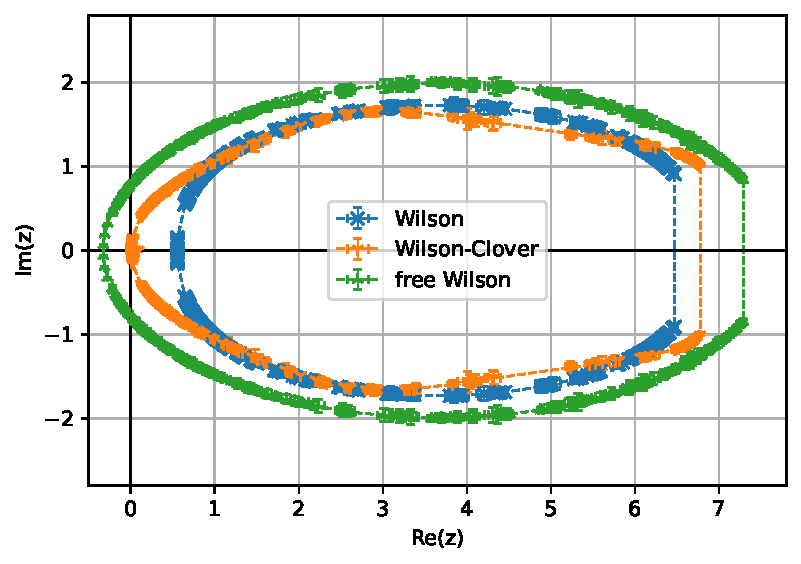
\includegraphics[width=0.47\textwidth]{\dir/img/sh/fine_sh}
    \label{fig:ch:fine}
}

\caption{
Boundary estimates of the numerical ranges (a) and spectral hulls (b) of the Wilson and Wilson-Clover Dirac operators.
}
\label{fig:fine}
\end{figure}

Numerical ranges of different coarse Wilson-Clover Dirac operators are plotted in \cref{fig:nr:coarse}.
\Cref{lemma:nr:xsym} suggests that the \case{1} case, \cref{fig:nr:coarse:case1}, should not show symmetry about the real axis, because the coarse operator is not $\Gamma^{5}$-Hermitian.
It is barely visible in the plots, but those numerical ranges are indeed \emph{not} symmetric, whereas the ones in \cref{fig:nr:coarse:case2,fig:nr:coarse:case6} are.
For a numerical verification of the numerical range and spectral hull symmetries, please refer to \cref{ch:appendix:symmetries}.

Furthermore the numerical range around the complex origin is related to the low mode subspace.
Thus, we want this regime to be well covered.
Comparing \cref{fig:nr:coarse:case2,fig:nr:coarse:case6} which correspond to \case{2,6} in \cref{tab:spins}, the coarse numerical range around the origin is identical (see insets), suggesting that keeping all \num{4} spins intact does not give any more benefit than just keeping the \num{2} chiralities intact.

\begin{figure}
\centering

\subfloat[\case{1}]{
    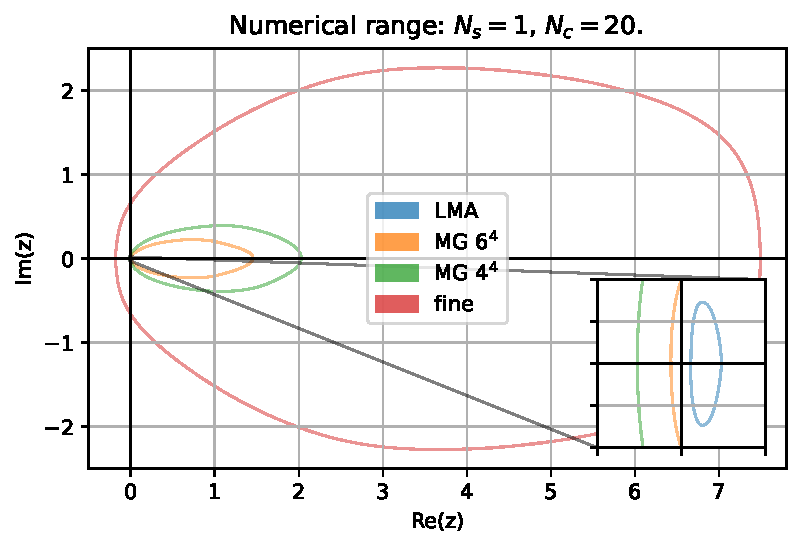
\includegraphics[width=0.47\textwidth]{\dir/img/nr/wc_Nc20_Ns1_nr}
    \label{fig:nr:coarse:case1}
}
\hfill
\subfloat[\case{2}]{
    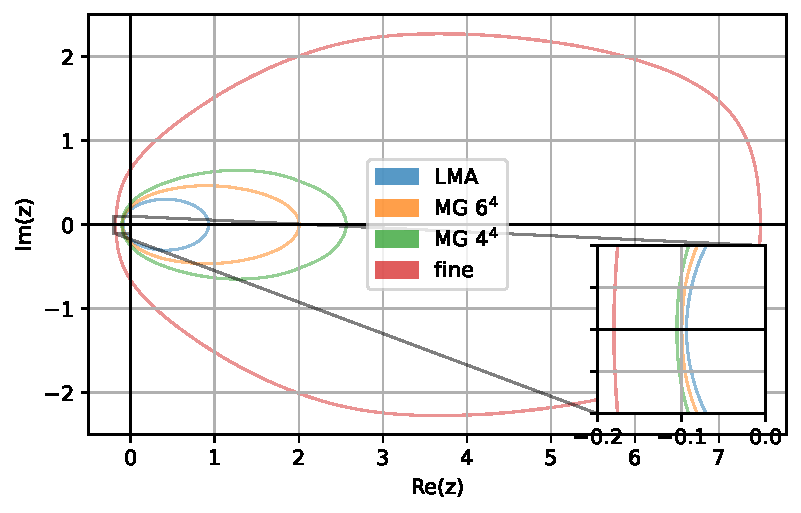
\includegraphics[width=0.47\textwidth]{\dir/img/nr/wc_Nc20_Ns2_nr}
    \label{fig:nr:coarse:case2}
}

\subfloat[\case{4}]{
    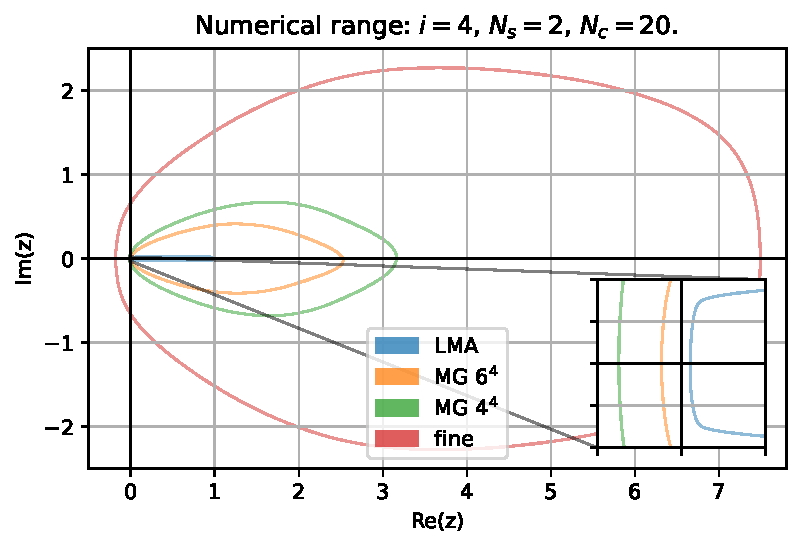
\includegraphics[width=0.47\textwidth]{\dir/img/nr/wc_Nc20_P02P13_nr}
    \label{fig:nr:coarse:case4}
}
\hfill
\subfloat[\case{6}]{
    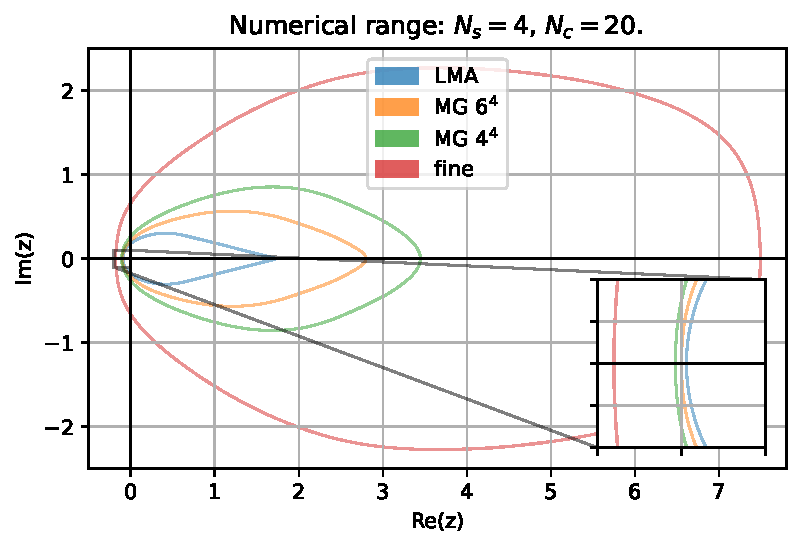
\includegraphics[width=0.47\textwidth]{\dir/img/nr/wc_Nc20_Ns4_nr}
    \label{fig:nr:coarse:case6}
}

\caption{
Numerical range boundary estimates of coarse and fine Wilson-Clover Dirac operators.
The subspaces were generated with $\Nc=20$ low modes of $\Gamma^{5} D$.
The panels correspond to spin projectors in \cref{tab:spins}.
Every panel shows different coarsening block sizes, where ``LMA'' corresponds to low-mode averaging, ``fine'' to the fine-grid operator and the MG aggregate block sizes are indicted in the labels.
}
\label{fig:nr:coarse}
\end{figure}

\section{Spectral hull}

We continue with studying the spectral hull, $\convshull{A}$, for fine and coarse Dirac operators.
According to \cref{thm:nr:properties}, the spectral hull is always contained in the numerical range of an operator.
For a non-normal operator they do not coincide, a comparing the areas of the numerical range and the spectral hull can be measure for non-normality.

We have determined the spectral hulls of the Wilson and Wilson-Clover Dirac operators \cref{fig:ch:fine} (see \cref{ch:appendix:nr:ch:estimator} for an algorithm).
Spectral hulls of different coarse Wilson-Clover Dirac operators are plotted in \cref{fig:ch:coarse}.
If chirality is preserved, we observe spectral hull inclusion from coarser to finer grids,
\begin{equation}
\convshull{\coarse{D}_{\text{LMA}}} \subseteq
\convshull{\coarse{D}_{6^{4}}} \subseteq
\convshull{\coarse{D}_{4^{4}}} \subseteq
\convshull{D_{\text{fine}}} \,.
\end{equation}
This is the strongest result of this section, because it makes coarse operators well conditioned
and immediately translates to condition numbers,
%and we immediately find $\kappa(\coarse{D}) \leq \kappa(D)$.
\begin{equation}
\kappa(\coarse{D}_{\text{LMA}}) \leq
\kappa(\coarse{D}_{6^{4}}) \leq
\kappa(\coarse{D}_{4^{4}}) \leq
\kappa(D_{\text{fine}}) \,.
\end{equation}
In \cref{fig:ch:coarse:case1}, this is not the case: all \num{3} coarse operators show eigenvalues in magnitude smaller than the smallest fine one.
This is a clear problem for numerical inversion.

To summarize, we collected condition numbers of relevant fine and coarse operators in \cref{tab:condition}.
Clearly the problem of spurious eigenvalues is not as severe for coarsenings of the non-Hermitian Dirac operator as compared to the Hermitian version, where the condition number explodes and thus becomes numerically inaccessible.
It is the smallest magnitude singular value (fourth column) responsible for the operators to become ill-conditioned as the highest one is capped by the maximal singular value on the fine grid.
For the \case{2} case, the smallest singular value is capped by the smallest one on the fine grid.
Empirically, we fine that chirality preservation leads to preservation of extremal eigen- and singular values.
For that reason, we considered the spectrum of the Hermitian Dirac operator in the next section.

\begin{figure}
\centering

\subfloat[\case{1}]{
    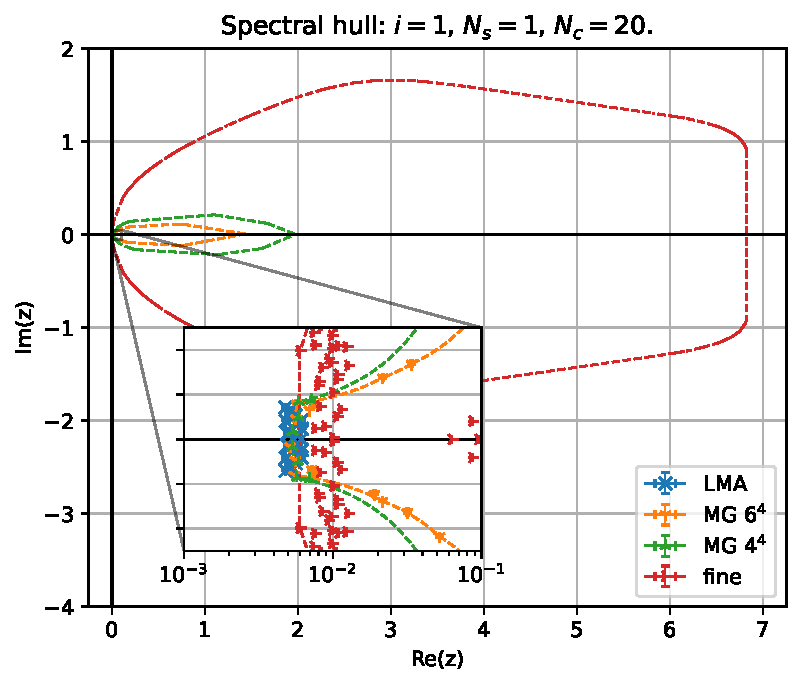
\includegraphics[width=0.47\textwidth]{\dir/img/sh/wc_Nc20_Ns1_sh}
    \label{fig:ch:coarse:case1}
}
\hfill
\subfloat[\case{2}]{
    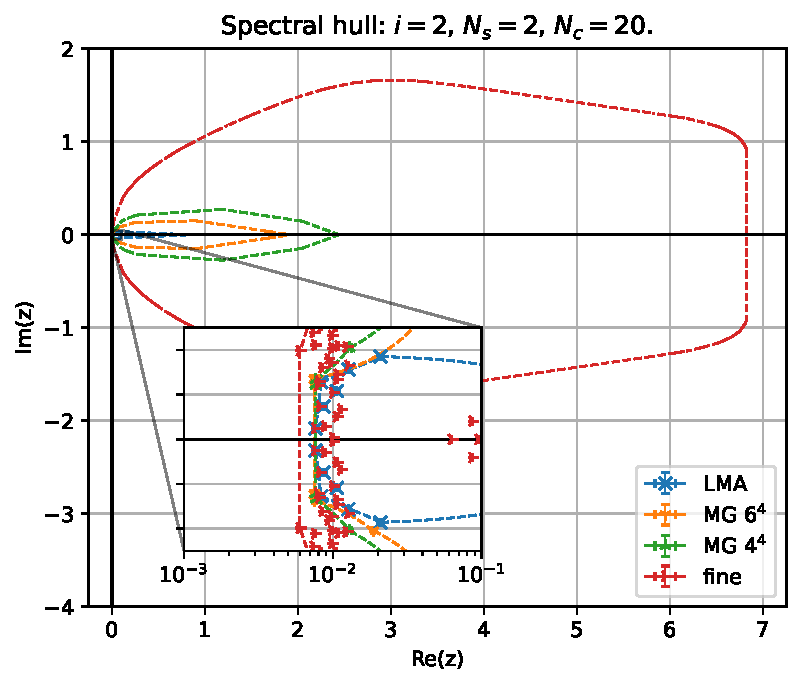
\includegraphics[width=0.47\textwidth]{\dir/img/sh/wc_Nc20_Ns2_sh}
    \label{fig:ch:coarse:case2}
}

\subfloat[\case{4}]{
    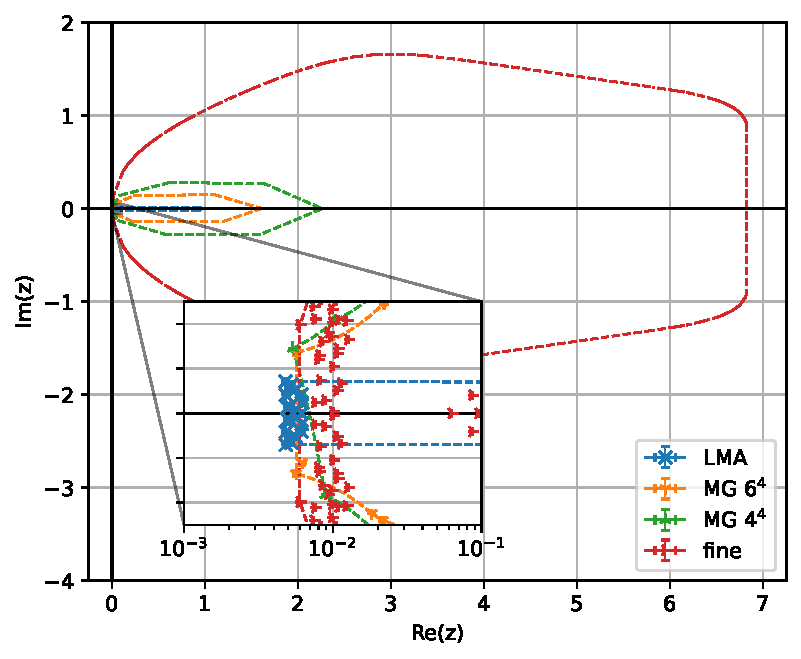
\includegraphics[width=0.47\textwidth]{\dir/img/sh/wc_Nc20_P02P13_sh}
    \label{fig:ch:coarse:case4}
}
\hfill
\subfloat[\case{6}]{
    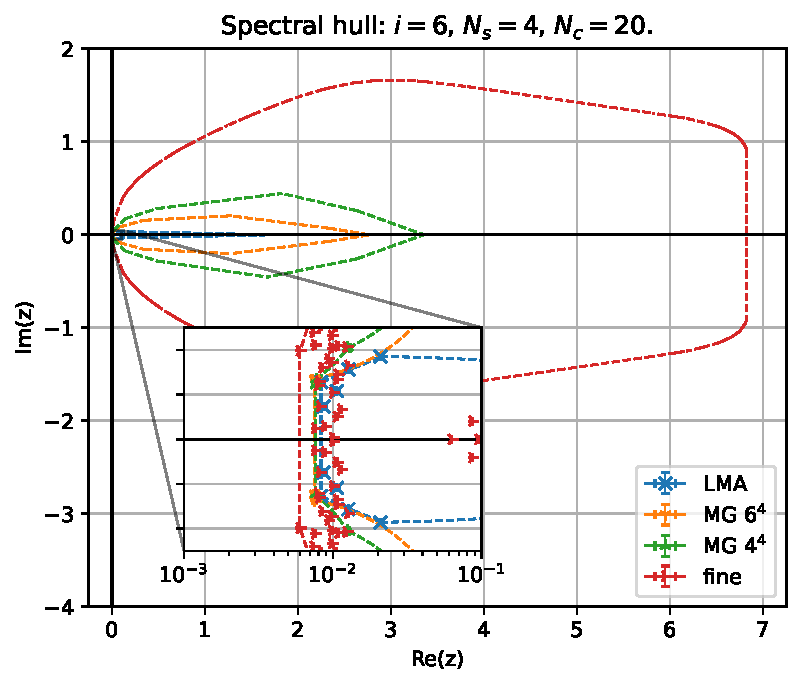
\includegraphics[width=0.47\textwidth]{\dir/img/sh/wc_Nc20_Ns4_sh}
    \label{fig:ch:coarse:case6}
}

\caption{
Spectral hull boundary estimates of coarse and fine Wilson-Clover Dirac operators.
This plots series corresponds to \cref{fig:nr:coarse}.
% The subspaces were generated with $\Nc=20$ low modes of $\Gamma^{5} D$.
% The panels correspond to spin projectors in \cref{tab:spins}.
% Every panels shows different coarsening block sizes, where ``no blocking'' corresponds to LMA and ``fine'' to the fine-grid operator.
Note that the inset x-axis is log-scale, meaning that the convex hull might not look convex, because the logarithm is a non-linear transformation.
}
\label{fig:ch:coarse}
\end{figure}

\newcommand{\nt}[2]{#1}
\newcommand{\ut}[2]{\underline{#1}}
\begin{table}
\begin{tabular}{ccc|cccc}
\toprule
Operator & Grid & Case & $\sigma_{min}(A)$ & $\sigma_{max}(A)$ & $\nrad{A}$ & $\kappa(A)$ \\
\midrule
$D_W, Q_W$ (free) & fine & -        & \nt{min}{x}
                                    & \nt{max}{x}
                                    & \nt{7.67}{7.667862627353456}
                                    & \nt{kappa}{x} \\
$D_W, Q_W$    & fine     & -        & \nt{0.435}{4.3549788925848770e-01}
                                    & \nt{7.17}{7.1730788452329097e+00}
                                    & \nt{7.11}{7.1108396881408895}
                                    & \nt{$16.5(0)$}{1.6470984181912677e+01} \\
$D_{WC}, Q_{WC}$ & fine  & -        & \nt{5.55e-3}{5.5481037267318730e-03}
                                    & \nt{7.65}{7.6462421529480125e+00}
                                    & \nt{7.49}{7.491162918196567}
                                    & \nt{$1380(20)$}{1.3781721700888340e+03} \\
\midrule
$\coarse{D}_{WC}$ & LMA  & \case{1} & \ut{4.18e-3}{4.1796137146807334e-03}
                                    & \nt{1.60e-2}{1.6013853253362759e-02}
                                    & \nt{1.55e-2}{0.015522532435122433}
                                    & \nt{$3.8(1)$}{3.8314194436473188e+00} \\
              & MG $6^4$ & \case{1} & \ut{4.44e-3}{4.4422207902965645e-03}
                                    & \nt{1.46}{1.4591063032306548e+00}
                                    & \nt{1.45}{1.4545971649705798}
                                    & \nt{$328(8)$}{3.2846325568010417e+02} \\
              & MG $4^4$ & \case{1} & \ut{4.54e-3}{4.5403408953169242e-03}
                                    & \nt{2.04}{2.0392773188336357e+00}
                                    & \nt{2.03}{2.028765960303842}
                                    & \nt{$450(10)$}{4.4914630109316721e+02} \\
\midrule
$\coarse{Q}_{WC}$ & LMA  & \case{1} & \nt{5.55e-3}{5.548102e-03}
                                    & \nt{2.31e-2}{2.312314e-02}
                                    & \nt{2.31e-2}{2.312314e-0,}
                                    & \nt{$4.16(7)$}{4.1677568292724} \\
              & MG $6^4$ & \case{1} & \ut{6.71e-4}{6.7129933376974750e-04 +/- 9.8931927945458135e-07}
                                    & \nt{1.08}{1.0840794144164108e+00 +/- 7.3226048798409186e-07}
                                    & \nt{1.08}{1.0840794144164108e+00 +/- 7.3226048798409186e-07}
                                    & \nt{$1615(2)$}{1.6148971999251899e+03 +/- 2.3799354798435797e+00} \\
              & MG $4^4$ & \case{1} & \ut{4.08e-5}{4.0847606195743720e-06 +/- 9.9131038427911789e-08}
                                    & \nt{1.58}{1.5680603876706616e+00 +/- 8.9749395241456465e-08}
                                    & \nt{1.58}{1.5680603876706616e+00 +/- 8.9749395241456465e-08}
                                    & \nt{$38(9) k$}{3.8388060738649894e+05 +/- 9.3162089010327891e+03} \\
\midrule
$\coarse{D}_{WC}, \coarse{Q}_{WC}$ & LMA  & \case{2}
                                    & \nt{5.55e-3}{5.5482402034070137e-03}
                                    & \nt{1.02}{1.0239883312989366e+00}
                                    & \nt{0.926}{0.9255000322214896}
                                    & \nt{$185(3)$}{1.8456092269944170e+02} \\
              & MG $6^4$ & \case{2} & \nt{5.55e-3}{5.5481098688822785e-03}
                                    & \nt{2.03}{2.0329543697857719e+00}
                                    & \nt{2.00}{2.003202952499008}
                                    & \nt{$366(6)$}{3.6642287514672643e+02} \\
              & MG $4^4$ & \case{2} & \nt{5.55e-3}{5.5481056289286559e-03}
                                    & \nt{2.59}{2.5881098949207302e+00}
                                    & \nt{2.56}{2.56364960063965}
                                    & \nt{$466(8)$}{4.6648533175466895e+02} \\
\midrule
$\coarse{D}_{WC}, \coarse{Q}_{WC}$ & LMA  & \case{5}
                                    & \nt{6.23e-2}{6.2289915389005336e-02}
                                    & \nt{1.67}{1.6752832371696156e+00}
                                    & \nt{1.67}{1.6752832371696156e+00}
                                    & \nt{26.9}{2.6894935186656497e+01} \\
              & MG $6^4$ & \case{5} & \nt{min}{x}
                                    & \nt{2.80}{2.7986287048257027}
                                    & \nt{2.80}{2.7986287048257027}
                                    & \nt{very ill}{x} \\
              & MG $4^4$ & \case{5} & \nt{min}{x}
                                    & \nt{max}{x}
                                    & \nt{nrad}{x}
                                    & \nt{very ill}{x} \\
\midrule
$\coarse{D}_{WC}, \coarse{Q}_{WC}$ & LMA  & PpP2P3
                                    & \nt{min}{x}
                                    & \nt{max}{x}
                                    & \nt{nrad}{x}
                                    & \nt{kappa}{x} \\
              & MG $6^4$ & PpP2P3   & \nt{min}{5.55e-3}
                                    & \nt{max}{2.7662710934964965}
                                    & \nt{nrad}{x}
                                    & \nt{kappa}{x} \\
              & MG $4^4$ & PpP2P3   & \nt{min}{x}
                                    & \nt{max}{x}
                                    & \nt{nrad}{x}
                                    & \nt{kappa}{x} \\
\midrule
$\coarse{D}_{WC}, \coarse{Q}_{WC}$ & LMA  & P0P2
                                    & \nt{min}{x}
                                    & \nt{max}{x}
                                    & \nt{nrad}{x}
                                    & \nt{kappa}{x} \\
              & MG $6^4$ & P0P2     & \nt{0.274}{2.7363581934309827e-01}
                                    & \nt{2.45}{2.4562335794482659e+00}
                                    & \nt{nrad}{x}
                                    & \nt{8.99}{8.9762867498297716e+00} \\
              & MG $4^4$ & P0P2     & \nt{0.256}{2.5563392568993265e-01}
                                    & \nt{3.05}{3.0528947892804035e+00}
                                    & \nt{nrad}{x}
                                    & \nt{11.9}{1.1942447705408892e+01} \\
\bottomrule
\end{tabular}
\caption{
Extremal singular values $\sigma_{min,max}(A)$, condition numbers $\kappa(A)$ and numerical radii $\nrad{A}$ for some coarse and fine, Hermitian and non-Hermitian Dirac operators.
$D_W$ and $D_{WC}$ indicate the Wilson and Wilson-Clover Dirac operators respectively and $Q$ is the Hermitian Dirac operator $Q = \Gamma^{5} D$.
For all coarsenings the $\Nc = 20$ lowest modes of $Q_{WC}$ were taken.
The underlined quantities are smallest singular values smaller than the fine grid one.
Associated operators are numerically problematic.
\worktodo{relative residual of 1e-9 for some}
}
\label{tab:condition}
\end{table}

\section{Numerical eigenvalue study}

To support our findings until now, we performed a spectral study of a Hermitian Wilson-Clover Dirac operator $\Gamma^{5} D$.
In this study, we generated multigrid subspaces in two different ways:
1) By naive coarsening corresponding to the \case{1} case in \cref{tab:spins} with $N_s=1$ remaining spins on the coarse grid.
2) By preserving chirality and the trace of $\Gamma^{5}$ corresponding to the \case{3} case with $N_s=2$ coarse spins.
\Cref{fig:chirality:spectrum} presents the results.

\begin{figure}
\centering
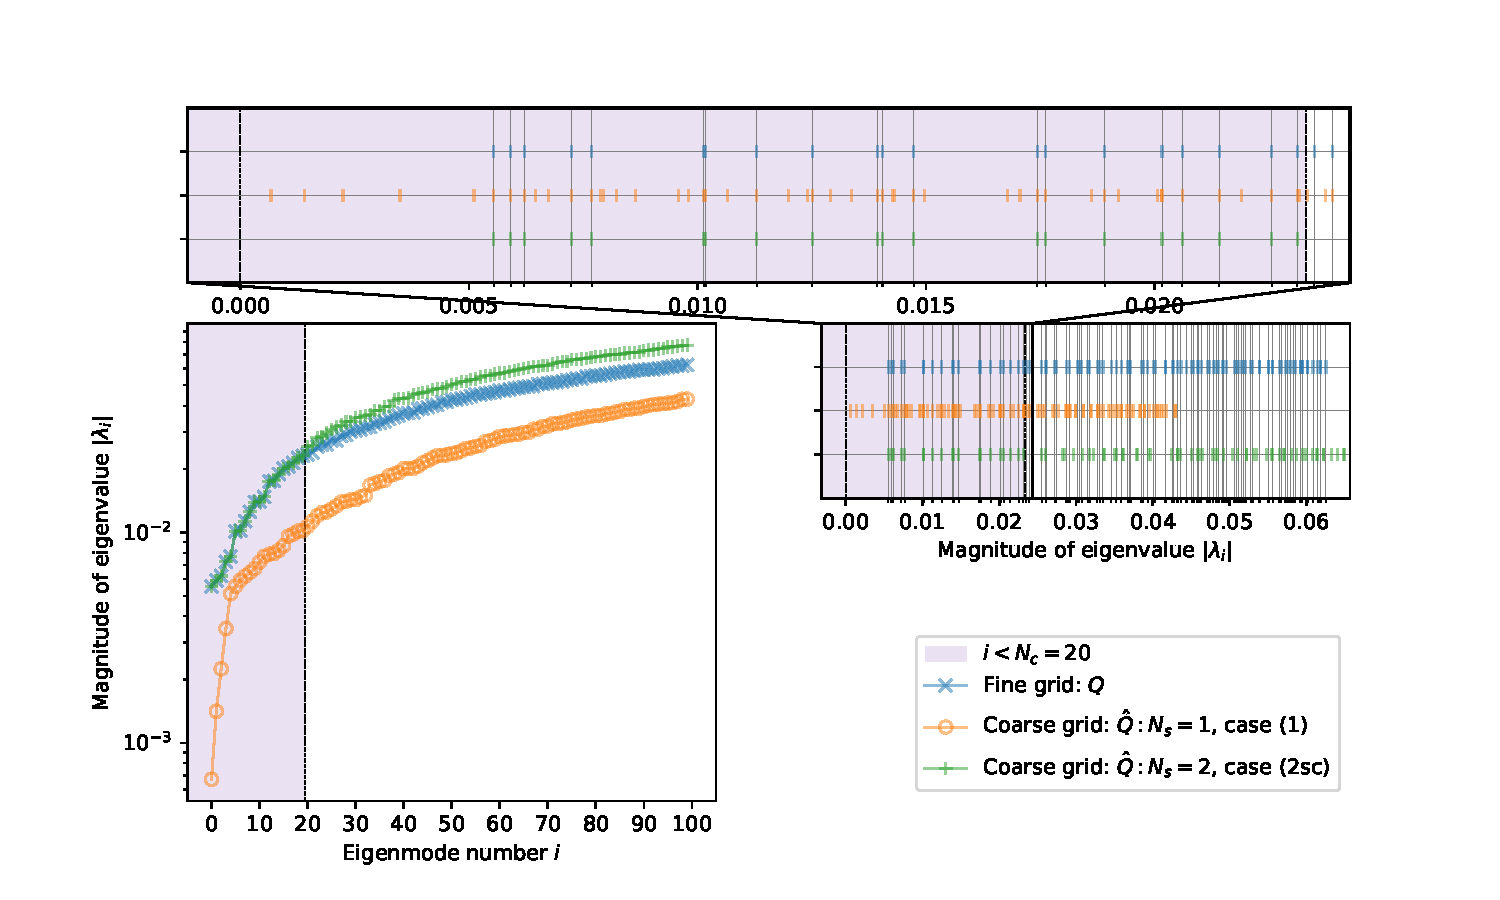
\includegraphics[width=1.0\linewidth]{\dir/img/eigenvalues_Nc20}
\caption{
Spectral study of coarse and fine Hermitian Dirac operators.
Lower left: eigenvalue magnitude versus mode number of the \num{100} lowest modes, lower right: eigenvalue magnitudes between find and different coarse operators for comparison, and top panel: zoom of lower right of the interesting region.
The three operators considered are fine (blue), coarse \case{1} (yellow) and coarse \case{3} (green), where $i$ corresponds to the row in \cref{tab:spins}.
\takenfull
}
\label{fig:chirality:spectrum}
\end{figure}

In blue the first \num{100} actual smallest-magnitude eigenvalues of the fine-grid Hermitian operator $Q = \Gamma^5 D$ are plotted.
The $\Nc=20$ smallest modes where taken to generate the coarse subspace for both scenarios.
For both coarse operators we also plotted their first \num{100} smallest-magnitude eigenvalues in yellow and green.
In the lower left panel their magnitudes are plotted, the top panel is a zoom of the lower right panel, which shows a tick for every eigenvalue at its magnitude for comparison.
On every fine-grid eigenvalue a grey vertical line is drawn for eye guidance.
The shaded region denotes the first \num{20} fine-grid modes for which we expect perfect overlap by construction for both coarse subspace as can be confirmed in the zoomed panel.

When coarsening all spins (yellow), we observe coarse eigenvalues lower than the lowest fine one as well as other spurious ones in the purple region.
These eigenvalues are responsible for ill-conditioned coarse systems and the slowing down of multigrid as a preconditioner as well as multigrid as variance reduction method introduced above.
On the other hand, when chiral properties are preserved (green), we cannot find a single eigenvalue in the critical purple region that is not an inherited one from the fine-grid.
Coarse eigenvalues above the purple region are distorted as expected, but they do not have impact in the condition.

\section{Numerical variance study}

The preserved chiral properties do not only have impact on the spectrum, but also the variance contribution of coarse subspaces.
\Cref{fig:chirality:variance} show how this presents itself.
We can clearly see an immense benefit from the chiral property preservation as opposed to its absence.
Variance contributing to the large distance regime therefore originates from both chiral sectors.
The yellow data corresponds to the \case{1} case in \ref{tab:spins}, whereas the green data to the \case{3} case.
Even though subspace of the \case{3} construction is twice as large as the \case{1} one, it is worth doing, not only for the condition of the coarse operator, but also for its variance contribution in the large distance.
\begin{figure}
\centering
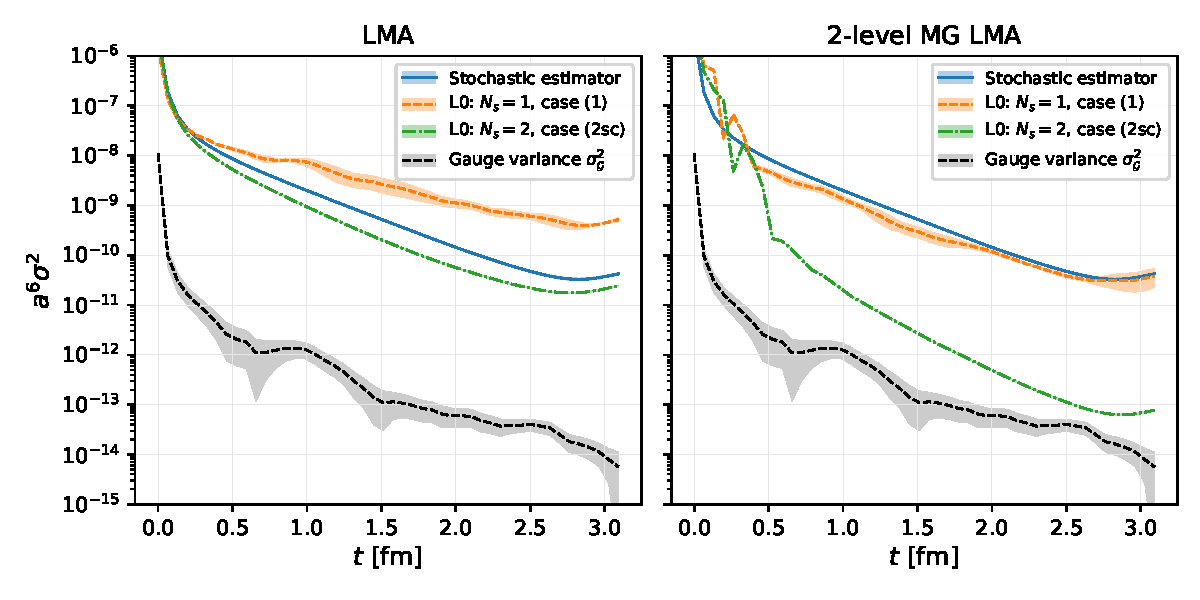
\includegraphics[width=1.0\linewidth]{\dir/img/chirality}
\caption{
Variance contribution of the \Ln{0}-term if all spin degrees of freedom are coarsened (yellow) as compared to when chiral properties are preserved (green).
Both LMA (left) and MG LMA (right) profit from these considerations.
\takenfull
}
\label{fig:chirality:variance}
\end{figure}


%\worktodo{plots with convex spectral hull, Ns2 Ns4 show spectral hull inclusion, Ns1 not!}
%\worktodo{table with areas and symmetry-metric.}

\section{Simple operators}



\textcolor{gray}{
\begin{theorem}[Condition of coarse normal, positively stable operators] \label{thm:cond:normal:pos:stable}
Assume $K$ to be a normal, $\Gamma^{5}$-Hermitian, positively stable ($\forall \lambda \in \sigma(B) \; : \; \Re{\lambda} > 0$) operator acting on the fine-grid lattice, $K \colon \vslattice \rightarrow \vslattice$, whose eigenvalue with smallest magnitude is real.
Then the condition number of the coarse-grid operator $\coarse{K}$ is bound from above by the condition number of the fine-grid operator,
\begin{equation}
\kappa(\coarse{K}) \leq \kappa(K) \;.
\end{equation}
\end{theorem}
}

\textcolor{gray}{
\begin{proof}
If $K$ is normal, its numerical range equals to the convex hull of its spectrum, $W(K) = \text{conv}\{\sigma(K)\}$, which in turn is symmetric about the real axis using \cref{lemma:nr:xsym}.
Thus $\sigma(\coarse{K}) \subseteq \text{conv}\{\sigma(K)\}$ and the element of smallest magnitude of $\text{conv}\{\sigma(K)\}$ is the real part of the eigenvalue of $K$ with smallest magnitude.
By assumption this eigenvalue is real.
Its largest element in magnitude is always smaller or equal to the eigenvalue of $K$ with largest magnitude.
Therefore $\kappa(\coarse{K}) \leq \kappa(K)$.
\end{proof}
}

\textcolor{gray}{
If the smallest magnitude eigenvalue of $K$ is not real, but complex in general, then the smallest magnitude element of $\text{conv}\{\sigma(K)\}$ is given by the real part of the smallest magnitude eigenvalue instead.
We then cannot guarantee anymore that the smallest magnitude eigenvalue of $\coarse{K}$ is not smaller than the one of $K$.
At least, we have the guarantee that $\coarse{K}$ is invertible, because $0 \not\in \text{conv}\{\sigma(K)\}$, a consequence of $K$ being positively stable.
}

\section{Final conjecture}

\textcolor{gray}{
We finish this chapter with a conjecture, motivated by the numerical and analytical studies above, from which we believe it is a sufficient condition for a well-behaved coarse-grid Dirac operator spectrum, suitable for coarse grid inversions as required by multigrid low-mode averaging.
\begin{conj}
Assume $K$ to be a positively stable, $\Gamma^{5}$-Hermitian operator acting on the fine-grid lattice, $K \colon \vslattice \rightarrow \vslattice$, not necessarily normal.
With Hermitian $P$ and $\Gamma^{5}$, we conjecture that if
\begin{equation} \label{eq:conj:chi}
\exists B \in \ggrp{GL}{N_s \Nc, \mathbb{C}} \; \colon \; \rho^5 = B \left( \chi^{5} \otimes \id_{\coarse{S}} \otimes \id_{\coarse{\idxcolor}} \right) B^{-1}
\end{equation}
for a change-of-basis matrix $B$, $\id_{\coarse{S}}$ is the identity of dimension either $1$ or $2$,
% and it holds
% \begin{equation} \label{eq:conj:modes}
% \forall i \; P \evec_i = \evec_i \;,
% \end{equation}
then chirality is preserved on the coarse lattice and
\begin{equation}
\kappa(\coarse{K}) \leq \kappa(K) \;.
\end{equation}
\end{conj}
}

\textcolor{gray}{
Additionally we demand invariance of the $N_c$ lowest eigenmodes
\begin{equation} \label{eq:conj:modes}
\forall i \; P \evec_i = \evec_i \;,
\end{equation}
since this is a requirement coming from low-mode averaging.
%The invariance of the eigenmodes \cref{eq:conj:modes} is a requirement coming from low-mode averaging.
If not satisfied the subspace will not include the exact low modes resulting in a degraded variance reduction compared to low-mode averaging.
The particular form of the coarse chirality operator \cref{eq:conj:chi} on the other hand fulfills the statements in \cref{lemma:chirality:preservation:equiv,lemma:chirality:preservation:implications,lemma:svd:coarse,lemma:evals:coarse} while preserving the trace.
}

\section{Summary}
\label{sec:chirality:summary}

The numerical range studies revealed important information about Wilson-type Dirac operators.
Critically, the Wilson-Clover operator is not accretive, even more so for physical masses, i.e. the operator itself, but also its coarse variants have the potential for zero or arbitrarily small modes in their spectra.
%We thus need a coarsening strategy that .
Empirically we observed spectral hull inclusion and perfect overlap of the $\Nc$ lowest modes for coarsening schemes that explicitly preserve chiral properties, no so for schemes that only preserve the non-chiral ones or none of the spins.
Therefore it is the chiral degree alone, that are responsible for well behaved spectra.
Spectral hull inclusion guarantees well-conditioned coarse operators, which is crucial for MG LMA and multigrid as a preconditioner to be beneficial.

Chirality on the coarse subspaces is an important concept. %, and critical for MG LMA and multigrid as a preconditioner to be beneficial.
We have seen multiple ways to achieve this, some of which are equivalent in their outcome.
We have studied the shapes of numerical ranges and spectral hulls of various coarse and fine Dirac operators.
The outcome was that for coarse operator spectra to behave well, we need to explicitly preserve fine-grid chirality.
The non-chiral spin degrees of freedom, if not preserved together with the chiral ones, still show smaller eigenvalues and lead to ill-conditioned coarse systems.
Also chiral indices have to be treated symmetrically to preserve the chiral operator trace.
Furthermore it is evident that the low-modes have to be perfectly represented in the subspace, else the variance reduction will be degraded.

For Hermitian positive definite systems, we are guaranteed to have a better conditioned coarse operator, no matter how we coarsen.
We systemically relaxed assumptions to the operator, still upholding this guarantee by studying their spectra. 
On this way, preserving spectral properties on coarse grids is crucial.
We believe that careful study of numerical range theory on lattice Dirac operators reveals further theoretic and algorithmic insights, also for other lattice discretizations.

\worktodo{todo}
